%!TEX TS-program = xelatex
\documentclass[]{friggeri-cv}
\usepackage{afterpage}
\usepackage{hyperref}
\usepackage{color}
\usepackage{xcolor}
\hypersetup{
    pdftitle={},
    pdfauthor={},
    pdfsubject={},
    pdfkeywords={},
    colorlinks=false,       % no lik border color
   allbordercolors=white    % white border color for all
}
\addbibresource{bibliography.bib}
\RequirePackage{xcolor}
\definecolor{pblue}{HTML}{0395DE}

\begin{document}
\header{Aaron}{Brooks/}{PhD}
      {\hspace{.2\textwidth} Genetics of complex adaptive biological systems}

% Fake text to add separator
\fcolorbox{white}{gray}{\parbox{\dimexpr\textwidth-2\fboxsep-2\fboxrule}{%
.....
}}

% In the aside, each new line forces a line break
\begin{aside}
  \section{Currently}
    \href{http://www.embl.de/research/units/genome_biology/steinmetz/}{Postdoc @ EMBL}
    ~
  \section{Mail}
    \href{mailto:aaron.brooks@embl.de}{\textbf{aaron.brooks@}\\embl.de}
    ~
    Steinmetz Lab
    Genome Biology Unit
    EMBL, Meyerhofstrasse 1
    69117 Heidelberg, Germany
    ~
  \section{Web}
    \href{http://www.aaron-brooks.org}{aaronbrooks.info}
    \href{https://www.linkedin.com/pub/aaron-brooks/17/774/3b3}{linkedin/aaron-brooks}
    \href{https://github.com/scalefreegan}{github/scalefreegan}
   ~
% \section{Tel \& Twitter}
   % +1 505 5064203
  \section{Twitter}
    \href{https://twitter.com/scalefreegan}{@scalefreegan}
    ~
    ~
    ~
    ~
    ~
    ~
    ~
    ~
    ~
    ~
    ~
    ~
    ~
    ~
    ~
    ~
%    \section{Research Breakdown}
%    ~
%    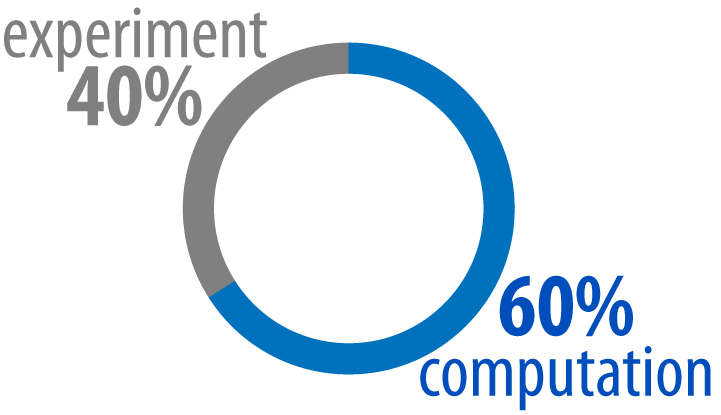
\includegraphics[scale=0.6]{img/breakdown.png}
    ~
\end{aside}

\section{Publications}
\href{http://journal.frontiersin.org/article/10.3389/fmicb.2015.00409/abstract}{\noindent
\textbf{AN Brooks}, WF Mueller, LM Steinmetz (2016)
\textbf{SYGNALing a Red Light for Glioblastoma.}
\emph{Cell Systems}  3 (2), 118-120
}
\\
\\
\href{http://journal.frontiersin.org/article/10.3389/fmicb.2015.00409/abstract}{\noindent
S Imam, S. Schaueble,  \textbf{AN Brooks}, NS Baliga, ND Price. (2015)
\textbf{Data-driven integration of genome-scale regulatory and metabolic network models.}
\emph{Front. Microbiol.} 6:409
}
\\
\\
\href{http://www.biomedcentral.com/1752-0509/8/122}{\noindent
CL Plaisier, FY Lo, J Ashworth, \textbf{AN Brooks}, KD Beer, A Kaur, M Pan, DJ Reiss, FT Facciotti, NS Baliga. (2014)
\textbf{Evolution of Context Dependent Regulation by Expansion of Feast/Famine Regulatory Proteins.}
\emph{BMC Systems Biology} 8(1):122.
}
\\
\\
\href{http://journal.frontiersin.org/article/10.3389/fmicb.2014.00379/abstract}{\noindent
H Westerhoff*, \textbf{AN Brooks*}, E Simeonidis*, R García-Contreras*, F Boogerd, F He, VJ Jackson, V Goncharuk, A Kolodkin. (2014)
\textbf{Macromolecular networks and intelligence in microorganisms.}
\emph{Front. Microbiol.} 5:379.
}
\\
\\
\href{http://msb.embopress.org/cgi/pmidlookup?view=long&pmid=25028489}{\noindent
\textbf{AN Brooks*}, DJ Reiss*, A Allard, W Wu, DM Salvanha, CL Plaisier, S Chandrasekaran, M Pan, A Kaur, NS Baliga.
\textbf{A system-level model for the microbial regulatory genome.}
\emph{Mol Syst Biol.} (2014) 10: 740.
}
\\
\\
\href{http://www.ncbi.nlm.nih.gov/pubmed/21197660}{\noindent
\textbf{AN Brooks}, S Turkarslan, KD Beer, FY Lo, NS Baliga. (2011)
\textbf{Adaptation of cells to new environments.}
\emph{Wiley Interdiscip Rev Syst Biol Med.} 3(5): 544–561.
}
\\
\\
$^{\ast}$ Denotes equal contribution

\section{Research}
\begin{entrylist}
  \entry
    {2015 - now}
    {Postdoc}
    {EMBL | Genome Biology Unit}
    {\emph{Project: ``Molecular consequences of large-scale genome variation in synthetic yeast.''}\\
    \emph{Advisors: Prof. Lars Steinmetz, Associate Head of Unit and Senior Scientist at EMBL, Dr. Oliver Stegle, Group leader at EMBL-EBI }\\}
\end{entrylist}

\section{Education}
\begin{entrylist}
  \entry
    {2008 - 2014}
    {PhD Molecular and Cellular Biology}
    {University of Washington}
    {\emph{Dissertation: ``Data-driven inference of dynamic transcriptional regulatory mechanisms in prokaryotes: a systems perspective.''}\\
    \emph{Advisor: Prof. Nitin Baliga, SVP and Director, Institute for Systems Biology}\\}
  \entry
    {2002 - 2007}
    {BS Biochemistry \& BA Political Science}
    {University of New Mexico}
    {\emph{Thesis: ``Characterization of the dynamic interactions of cytoplasmic poly(A) binding protein with poly(A) RNA.''}\\
    \textit{Thesis Honors: Robert B. Loftfield Award}\\
    \emph{Advisor: Prof. David G. Bear}\\
    \textit{Summa Cum Laude}\\
    \textit{General University Honors}\\
    \textit{Minor: Philosophy}}
\end{entrylist}
\newpage
\section{In the news}
\begin{entrylist}
  \entry
    {05/2014}
    {\href{http://publications.nigms.nih.gov/insidelifescience/knowing-networks.html}{Knowing Networks}}
    {NIH NIGMS Inside Life Science}
    {\emph{Outreach at USA Science and Engineering Festival}}
\end{entrylist}

\section{Awards}
\begin{entrylist}
   \entry
    {2016-2019}
    {EMBL Interdisciplinary Postdoctoral Fellowship (EIPOD)}
    {EU Marie Curie Actions}
    {}
  \entry
    {2010-2013}
    {Office of Science Graduate Fellowship}
    {Department of Energy}
    {}
   \entry
    {2006}
    {Goldwater Scholarship}
    {Barry M. Goldwater Foundation}
    {}
\end{entrylist}

% In the aside, each new line forces a line break
\begin{aside}
~
~
~
~
~
\section{Research Interests}
     ~
    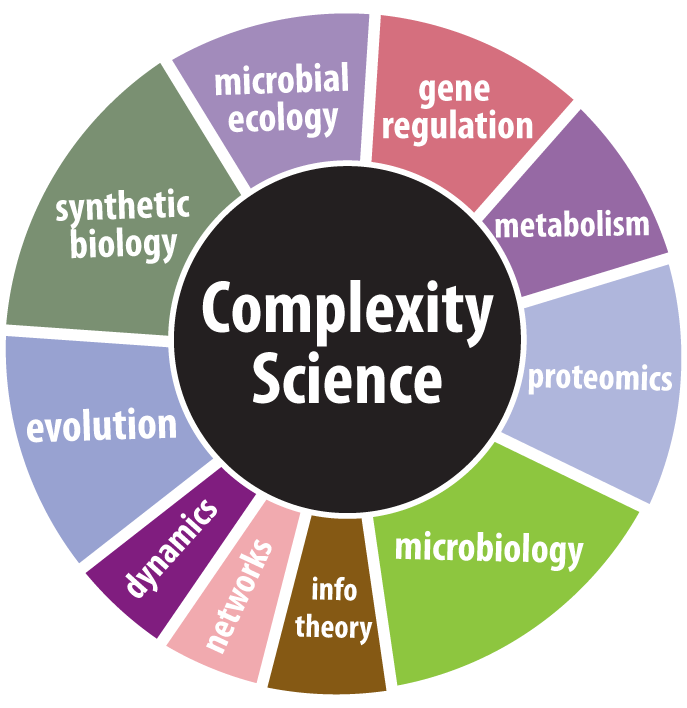
\includegraphics[scale=0.6]{img/interests.png}
    ~
\section{Wetlab}
    \textbf{MolBio}
\includegraphics[scale=0.40]{img/5stars.png}
    \textbf{Sequencing}
\includegraphics[scale=0.40]{img/5stars.png}
    \textbf{Bioreactor}
\includegraphics[scale=0.40]{img/4stars.png}
    \textbf{Microscopy}
\includegraphics[scale=0.40]{img/2stars.png}
    ~
  \section{Programming}
    \textbf{R}
\includegraphics[scale=0.40]{img/5stars.png}
    \textbf{Python}
\includegraphics[scale=0.40]{img/5stars.png}
    \textbf{Bash}
\includegraphics[scale=0.40]{img/4stars.png}
    \textbf{HTML/JS}
\includegraphics[scale=0.40]{img/4stars.png}
    \textbf{SQL}
\includegraphics[scale=0.40]{img/3stars.png}
    \textbf{Malab}
\includegraphics[scale=0.40]{img/3stars.png}
     \textbf{C++}
\includegraphics[scale=0.40]{img/1stars.png}
    ~
  \section{Research Summary}
    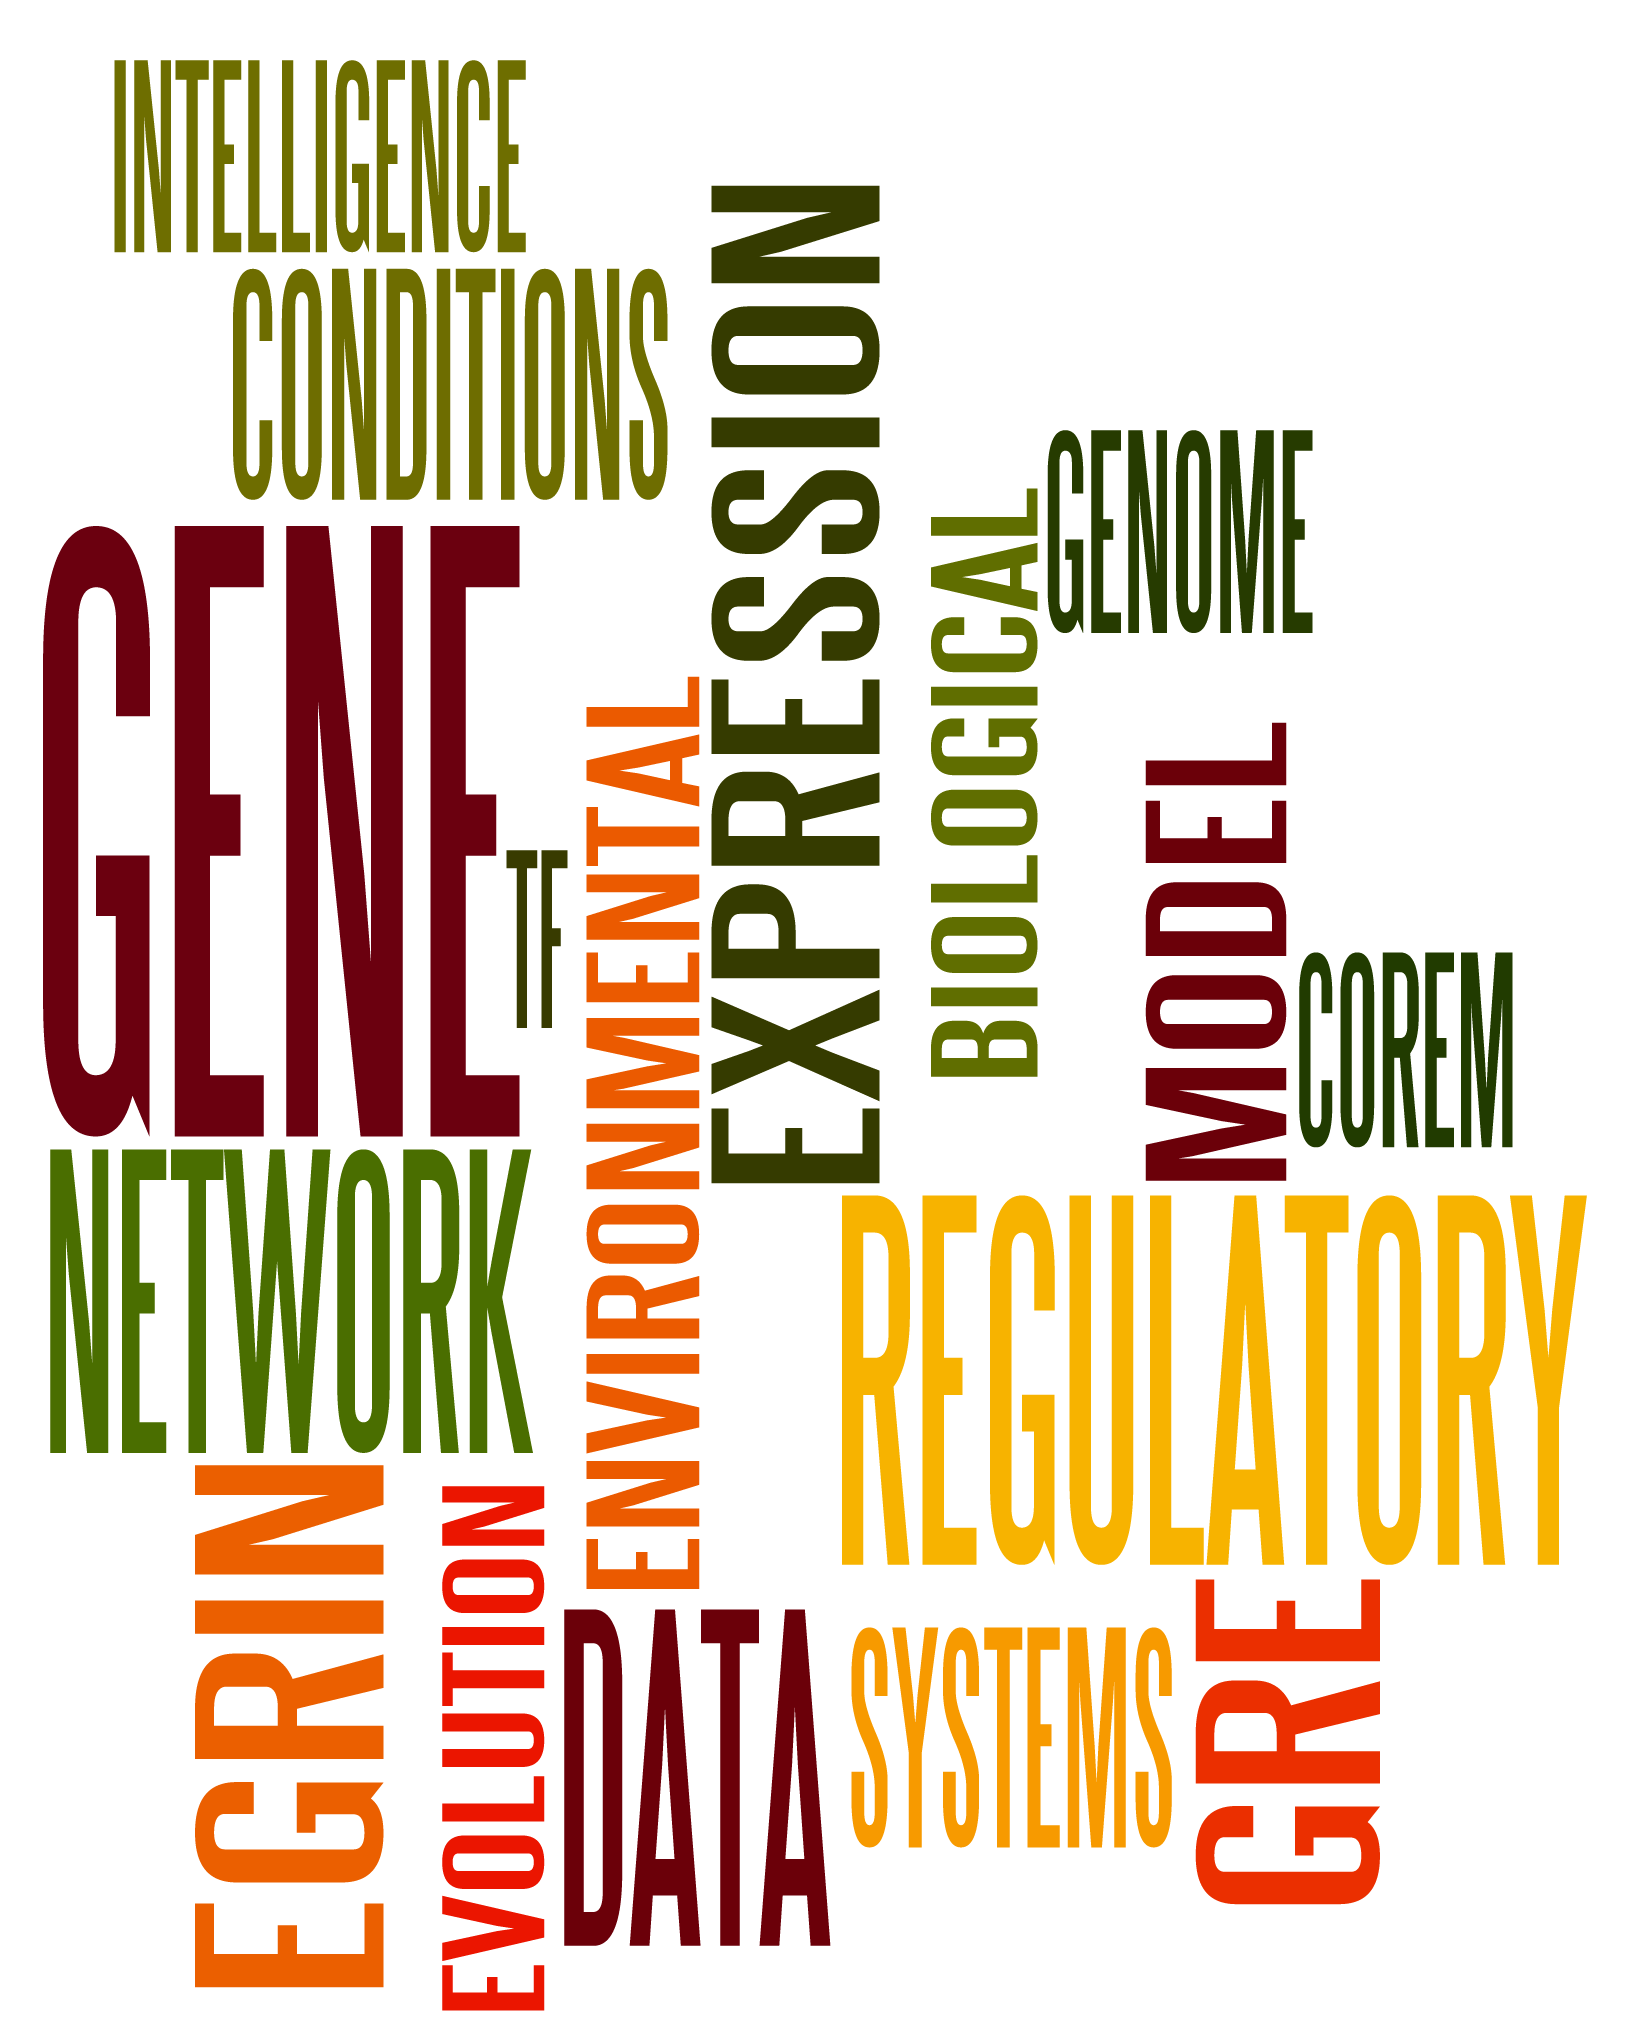
\includegraphics[scale=0.28]{img/wordle_small.png}
    ~
\end{aside}

\section{Teaching \& Outreach}
\begin{entrylist}
    \entry
    {2015}
    {\href{http://scalefreegan.github.io/Teaching/DataIntegration/}{EMBL: Data Mining and Integration with Networks}}
    {Heidelberg, Germany}
    {\emph{Co-organizer, lecturer}}
  \entry
    {2014}
    {USA Science and Engineering Festival}
    {Washington, D.C}
    {\emph{Designed and facilitated a hands-on activity and web-based game to understand the structure and function of networks. Over 300 students have played the online game.}}
  \entry
    {2011}
    {Introduction to Systems Biology}
    {Institute for Systems Biology}
    {\emph{Co-organizer, lecturer}}
    \entry
    {2009-2015}
    {Science Communication Fellow}
    {Pacific Science Center, Seattle WA}
    {}
%    \entry
%    {2010}
%    {Graduate Teaching Assistant}
%    {Microbiology, University of Washington}
%    {\emph{MICRO 411: Gene Action}}
%    \entry
%    {2005-2006}
%    {Education Assistant}
%    {Biochemistry, University of New Mexico}
%    {\emph{BIOCHEM 445: Intensive Biochemistry}\\
%    \emph{BIOCHEM 448: Biochemical Methods}}
\end{entrylist}

\section{Students mentored}
\begin{entrylist}
  \entry
    {08-12/2012}
    {Robin Green}
    {PhD student at University of Washington, WA}
    {Currently at Fred Hutchinson Cancer Research Center}
  \entry
    {05-08/2011}
    {Darach Miller}
    {Undergraduate at UC Davis, CA}
    {Currently PhD student at NYU}
  \entry
    {05-08/2010}
    {Alexis Valauri-Orton}
    {Undergraduate at Davidson College, NC}
    {Currently ‎Ocean Acidification Intern at Ocean Conservancy}
\end{entrylist}

\section{Other}
\begin{entrylist}
 \entry
    {2011}
    {Complex Systems Summer School}
    {Santa Fe Institute}
    {}
  \entry
    {2010}
    {MCB Student Symposium}
    {Fred Hutchinson Cancer Research Center}
    {Co-organizer, \emph{Bioplasticity: flexibility within and beyond the code}}
\end{entrylist}
\newpage
\section{References}
\begin{entrylist}
\entry
    {}
    {Lars Steinmetz, PhD}
    {EMBL / Stanford}
    {+49 6221 387389\\
    \href{mailto:larsms@embl.de}{\textbf{larsms}@embl.de}}
    \entry
    {}
    {Nitin Baliga, PhD}
    {Institute for Systems Biology}
    {+1 206 7321266\\
    \href{mailto:nbaliga@systemsbiology.org}{\textbf{nbaliga@}systemsbiology.org}}
     \entry
    {}
    {Oliver Stegle, PhD}
    {EMBL-EBI}
    {+44 1223 494101\\
    \href{mailto:stegle@ebi.ac.uk}{\textbf{stegle@}ebi.ac.uk}}
     \entry
     {}
    {Patrick Cai, PhD}
    {University of Manchester}
    {+44 161 3064214\\
    \href{mailto:yizhi.ca@manchester.ac.uk}{\textbf{yizhi.ca@}manchester.ac.uk}}
     \entry
    {}
    {Elhanan Borenstein, PhD}
    {University of Washington}
    {+1 206 6858165\\
    \href{mailto:elbo@uw.edu}{\textbf{elbo@}uw.edu}}
\end{entrylist}

\end{document}
